\subsubsection{Affichage en ligne de commande}

Le projet inclut également deux fonctions d'affichage dans \texttt{io.jl}, conformément à la partie demandée sur la visualisation en console :
\begin{itemize}
    \item \texttt{displayGrid()}, qui affiche une instance non résolue ;
    \item \texttt{displaySolution()}, qui affiche une solution obtenue à partir des variables de palissades.
\end{itemize}

Dans notre cas, ces fonctions ont été testées sur l'instance \texttt{instanceTest.txt}. La Figure~\ref{fig:palisade-console-display} montre d'abord l'affichage de la grille initiale, puis l'affichage de la solution reconstruite en console.

\begin{figure}[H]
    \centering
    \begin{subfigure}[t]{0.48\textwidth}
        \centering
        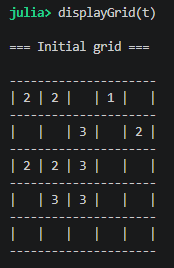
\includegraphics[width=\textwidth]{imgs/palisade_display.png}
        \caption{Affichage de l'instance non résolue avec \texttt{displayGrid()}.}
    \end{subfigure}
    \hfill
    \begin{subfigure}[t]{0.48\textwidth}
        \centering
        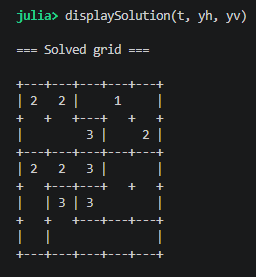
\includegraphics[width=\textwidth]{imgs/palisade_display_solution.png}
        \caption{Affichage de la solution avec \texttt{displaySolution()}.}
    \end{subfigure}
    \caption{Visualisation en ligne de commande pour \textit{Palisade}.}
    \label{fig:palisade-console-display}
\end{figure}
